\documentclass{article}
\usepackage[utf8]{inputenc}
\usepackage{geometry}
\usepackage{hyperref}
 \geometry{
 a4paper,
 total={170mm,257mm},
 left=20mm,
 top=20mm,
 }
 \usepackage{graphicx}
 \graphicspath{{Pics/}}
 \usepackage{titling}
 \title{Inequality in the Economy: Testing Piketty's Theory through Simulation
}
\author{Haoran Jie hj376}
\date{January 2023}
 
 \usepackage{fancyhdr}
\fancypagestyle{plain}{%  the preset of fancyhdr 
    \fancyhead[L]{Tick4}
    \fancyhead[R]{\theauthor}
    \fancyfoot[C]{} % Add this line to remove the page number
}
\makeatletter
\def\@maketitle{%
  \newpage
  \null
  \vskip 0.3em%
  \begin{center}%
  \let \footnote \thanks
    {\LARGE \@title \par}%
    \vskip 0.8em%
    %{\large \@date}%
  \end{center}%
  \par
  \vskip 0.3em}
\makeatother

\usepackage{lipsum}  
\usepackage{cmbright}

\begin{document}

\maketitle


\section*{Goals}
Argued by the economist Thomas Piketty in his book \textit{Capital in the Twenty-first Century}, the growth of income from capital (i.e. investments, property, etc.)\footnote{This study simplifies the situation by assuming capital to be the current wealth} has been outpacing economic growth, leading to increased inequality. This report gather, simulate, and analyse data to test the validity of Piketty's theory and to understand the causes and implications of increasing inequality.
\vspace{-0.4cm}
\section*{Methodology}
\vspace{-0.3cm}
To test Thomas Piketty's theory, this study will simulate the economy by 
assigning each individual\footnote{1000 individuals, and 100 timesteps in total} a random, normally-distributed, per-timestep income and calculating the return on capital by multiplying wealth $w_i$ by a growth 
factor $g_i$ every timestep.\footnote{$g_i$ is calculated such that it positively correlates with $w_i$, and the total return to capital would approximately match the ratio} The simulator will normalize wealth every timestep, by limiting total with to 1000, to prevent numerical instability. The results of the 
simulation will be measured by the Gini coefficient, which will indicate the level of inequality in the distribution of wealth,
 and by a mobility measure, which will calculate the proportion of individuals who moved more than one quintile. By comparing 
 the results of simulations with different ratios of return on capital to growth due to income, the report will seek to 
 understand the relationship between the two and the validity of Piketty's theory.\footnote{Source code is made available on  \url{https://github.com/Haoran-Jie/EconomicInequality_Simulator_Investigation}}


\vspace{-0.4cm}



% 1000 individuals randomly assigned per-timestep income
% Return on capital growth factor
% Gini coeficient to measure inequality
% Also measure economic mobility because "some degree of inequality might be acceptible if economic mobility were high"
% Incorporate exchange model to allow for certain level of uncertainty (The extension for tick 1)\\

\section*{Result}
\vspace{-0.3cm}

Our plot on the left shows that as the ratio of return on capital to growth due to income increases, 
the Gini coefficient also increases as iteration goes through, indicating higher levels of inequality. \\
Our plot on the right shows that there exists an inverse relationship between mobility and the ratio of return on capital to growth due to income increases, despite some fluctuations. 

\vspace{0.3cm}
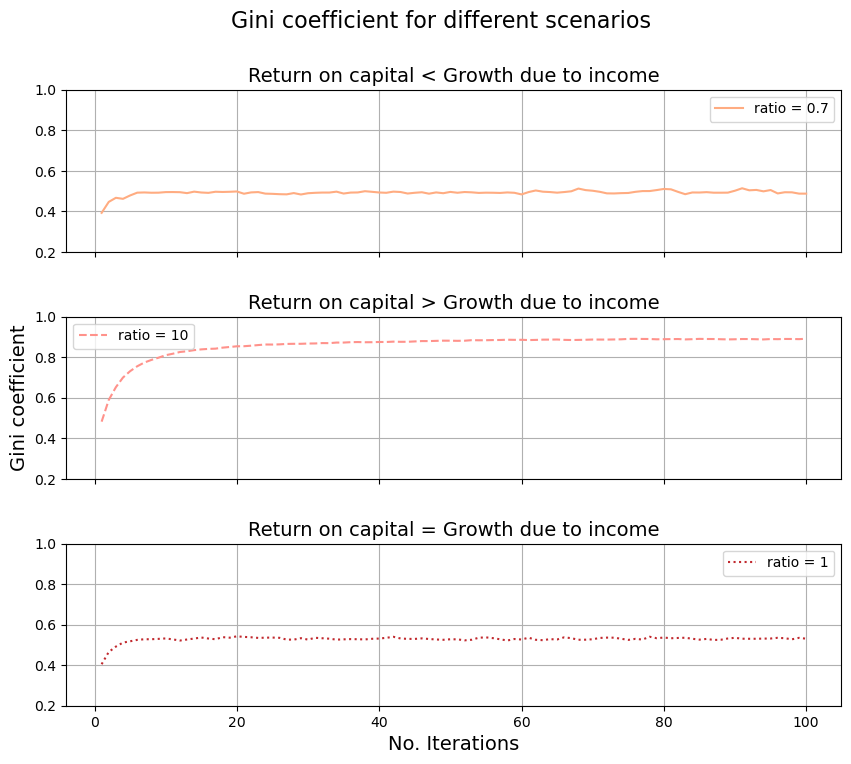
\includegraphics[width=8cm,height=7cm]{ratio_comparison.png}
\hspace{0.2cm}
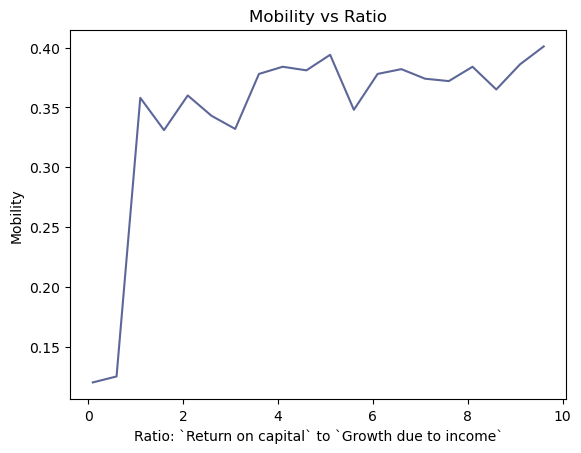
\includegraphics[width=8cm,height=7cm]{Mobility.png}

\vspace{-0.4cm}
\section*{Conclusion}
The conclusion of this report supports Thomas Piketty's theory that increased inequality in the economy is due to a higher
return on capital than income growth.
The results of the simulations indicate that this leads to decreased mobility and increased 
concentration of wealth in a few individuals. It is interesting to see that the gradient of the curve decreases and will eventual reach a limit as a horiontal asymptotes. The findings of this report suggest the need for policies to 
address the issue of increasing inequality in the economy.

\end{document}
